% \iffalse meta-comment
%
% Copyright (C) 2006 by Scott Pakin <scott+ctip@pakin.org>
% --------------------------------------------------------
%
% This file may be distributed and/or modified under the
% conditions of the LaTeX Project Public License, either version 1.3b
% of this license or (at your option) any later version.
% The latest version of this license is in:
%
%    http://www.latex-project.org/lppl.txt
%
% and version 1.3b or later is part of all distributions of LaTeX
% version 2006/01/07 or later.
%
% \fi
%
% \iffalse
%<*driver>
\ProvidesFile{cooltooltips.dtx}
%</driver>
%<package>\NeedsTeXFormat{LaTeX2e}[2001/06/01]
%<package>\ProvidesPackage{cooltooltips}
%<*package>
    [2006/03/07 v1.0 Cool PDF tooltips]
%</package>
%
%<*driver>
\documentclass{ltxdoc}
\usepackage{cooltooltips}
\usepackage{graphicx}
\usepackage{color}
\usepackage{hyperref}
\EnableCrossrefs
\CodelineIndex
\RecordChanges
\begin{document}
  \sloppy
  \DocInput{cooltooltips.dtx}
%  \PrintChanges
  \PrintIndex
\end{document}
%</driver>
% \fi
%
% \CheckSum{204}
%
% \CharacterTable
%  {Upper-case    \A\B\C\D\E\F\G\H\I\J\K\L\M\N\O\P\Q\R\S\T\U\V\W\X\Y\Z
%   Lower-case    \a\b\c\d\e\f\g\h\i\j\k\l\m\n\o\p\q\r\s\t\u\v\w\x\y\z
%   Digits        \0\1\2\3\4\5\6\7\8\9
%   Exclamation   \!     Double quote  \"     Hash (number) \#
%   Dollar        \$     Percent       \%     Ampersand     \&
%   Acute accent  \'     Left paren    \(     Right paren   \)
%   Asterisk      \*     Plus          \+     Comma         \,
%   Minus         \-     Point         \.     Solidus       \/
%   Colon         \:     Semicolon     \;     Less than     \<
%   Equals        \=     Greater than  \>     Question mark \?
%   Commercial at \@     Left bracket  \[     Backslash     \\
%   Right bracket \]     Circumflex    \^     Underscore    \_
%   Grave accent  \`     Left brace    \{     Vertical bar  \|
%   Right brace   \}     Tilde         \~}
%
%
% \changes{v1.0}{2006/03/07}{Initial version}
%
% \GetFileInfo{cooltooltips.dtx}
%
% \DoNotIndex{\@ifundefined,\@tempboxa,\@tempcnta,\@tempcntb}
% \DoNotIndex{\@tempdima,\@tempdimb,\@tempdimc,\\}
% \DoNotIndex{\active,\addtolength,\advance}
% \DoNotIndex{\begingroup,\bgroup}
% \DoNotIndex{\catcode,\csname}
% \DoNotIndex{\DeclareRobustCommand,\def,\dp}
% \DoNotIndex{\edef,\egroup,\else,\endcsname,\endgroup,\expandafter}
% \DoNotIndex{\fi}
% \DoNotIndex{\gdef}
% \DoNotIndex{\hbox,\hspace,\ht}
% \DoNotIndex{\ifnum,\ifpdf,\immediate}
% \DoNotIndex{\let}
% \DoNotIndex{\makebox,\mbox,\MessageBreak}
% \DoNotIndex{\newcommand,\noexpand}
% \DoNotIndex{\paperwidth,\pdflastannot,\pdflastobj,\pdflastxform}
% \DoNotIndex{\renewcommand}
% \DoNotIndex{\savebox,\setbox,\setcounter,\setlength,\space}
% \DoNotIndex{\stepcounter,\strip@pt}
% \DoNotIndex{\the,\thepage}
% \DoNotIndex{\usebox}
% \DoNotIndex{\wd}
% \DoNotIndex{\xdef}
%
% ^^A  Define the document's metadata.
% \title{The \cool\ package\thanks{This document
%   corresponds to \textsf{cooltooltips}~\fileversion, dated \filedate.}}
% \author{Scott Pakin \\ \texttt{scott+ctip@pakin.org}}
% \hypersetup{^^A
%   pdftitle={The cooltooltips package},
%   pdfauthor={Scott Pakin <scott+ctip@pakin.org>},
%   pdfsubject={Including cool-looking tooltips in a pdfLaTeX document},
%   pdfkeywords={tooltips, popups, pdfLaTeX, LaTeX package, PDF}
% }
%
% ^^A  Define some logical styles and helper macros to use throughout
% ^^A  the documentation.
% \let\acro=\textsc
% \newcommand*{\pdfterm}[1]{\textsf{#1}}
% \let\pkgname=\textsf
% \newcommand*{\cool}{\pkgname{cooltooltips}}
%
% ^^A  The following definition was copied more-or-less verbatim
% ^^A  from ltxguide.cls.
% \makeatletter
% \DeleteShortVerb{\|}
% \newenvironment{decl}
%     {\par\small\addvspace{4.5ex plus 1ex}^^A
%      \vskip -\parskip
%      \noindent\hspace{-\leftmargini}^^A
%      \begin{tabular}{|l|}\hline\ignorespaces}^^A
%     {\\\hline\end{tabular}\nobreak\par\nobreak
%      \vspace{2.3ex}\vskip -\parskip}
% \MakeShortVerb{\|}
% \makeatother
%
% ^^A  The following were copied blindly from the UK TeX FAQ.
% \renewcommand{\topfraction}{.85}
% \renewcommand{\bottomfraction}{.7}
% \renewcommand{\textfraction}{.15}
% \renewcommand{\floatpagefraction}{.66}
% \renewcommand{\dbltopfraction}{.66}
% \renewcommand{\dblfloatpagefraction}{.66}
% \setcounter{topnumber}{9}
% \setcounter{bottomnumber}{9}
% \setcounter{totalnumber}{20}
% \setcounter{dbltopnumber}{9}
%
%
% \maketitle
%
% \section{Introduction}
%
% The \cool\ package enables a document to contain hyperlinks that pop
% up a brief tooltip when the mouse moves over them and also open a
% small window containing additional text.  \cool\ works only with
% pdf\LaTeX\@.  Furthermore, the tooltips that \cool\ produces are much
% less cool when viewed under older versions of Acrobat~($<7.0$) or the
% current version of xpdf~(3.00) because they don't pop up the extra,
% small window.  \cooltooltip[0 0 1]{Example}{This is an example of a
% cool tooltip.  Pretty cool, eh?}{http://www.ctan.org/}{Visit CTAN on
% the Web}{This text\strut} is an example of a cool tooltip (assuming
% you're viewing this document with a sufficiently capable \acro{pdf}
% reader).  Move your mouse pointer over it and watch what happens.
% Then, click on the link.  If your \acro{pdf} reader is properly
% configured it should launch a Web browser and send it to the
% \acro{ctan} home page.
%
% If the \cool\ popup mechanism causes problems with your browser you
% can \cooltooltiptoggle{\fcolorbox{blue}{white}{click here}} to disable
% popups.  (Click again to re-enable them.)  Regardless of whether
% popups are enabled the tooltip and hyperlink mechanisms continue to
% function.
%
% The cool tooltip shown above was created with the following code:
%
% \begin{verbatim}
%     \cooltooltip
%       [0 0 1]
%       {Example}
%       {This is an example of a cool tooltip. Pretty cool, eh?}
%       {http://www.ctan.org/}{Visit CTAN on the Web}
%       {This text\strut}
% \end{verbatim}
%
% The ``click here'' button was created as follows:
%
% \begin{verbatim}
%     \cooltooltiptoggle{\fcolorbox{blue}{white}{click here}}
% \end{verbatim}
%
%
% \section{Usage}
%
% \begin{decl}
%   \texttt{\string\cooltooltip} \oarg{popup color} \oarg{link color} \\
%   \marg{subject} \marg{message} \marg{\acro{url}} \marg{tooltip}
%   \marg{text}
% \end{decl}
% \bgroup
%   \def\PrintDescribeMacro#1{}
%   \DescribeMacro{\cooltooltip}
% \egroup
% The |\cooltooltip| macro takes two optional arguments and five
% mandatory arguments.  The first argument, \meta{popup color}, is the
% color of the box containing the textual message to display and is
% specified as a ``\meta{red} \meta{green} \meta{blue}'' triple with
% each element ranging from 0~(off) to 1~(on).  If omitted, \meta{popup
% color} defaults to ``\texttt{0 1 0}''~(bright green).  The second
% argument, \meta{link color}, is the color of the frame drawn around
% the hyperlink.  If omitted, it defaults to the same value as
% \meta{popup color}.  \meta{subject} is a text string to display as the
% subject of the popup window.  \meta{message} is a text string to
% display within the popup window.  There's no provision for scrolling
% the popup window so \meta{message} should be kept reasonably short.
% When a user clicks on the hyperlink, the \acro{pdf} browser should
% take him to \acro{url} \meta{\acro{url}}.  While the mouse is hovering
% over the link, the \meta{tooltip} text is displayed.  Finally,
% \meta{text} is the text of the hyperlink and can be composed of
% arbitrary \LaTeX\ text, including mathematics, graphics, etc.
%
% The width of the hyperlink frame is governed by |\fboxrule| and the
% space separating the frame from \meta{text} is governed by |\fboxsep|.
% Use \LaTeX's |\setlength| command to assign values to those registers.
%
% Figure~\ref{fig:ctip-arguments} illustrates how Adobe Reader~7.0
% displays \meta{subject}, \meta{message}, \meta{tooltip}, and
% \meta{text} with a \meta{popup color} of cyan (\texttt{0 1 1}) and a
% \meta{link color} of magenta (\texttt{1 0 1}).  (The \acro{url}
% specified by \meta{\acro{url}} does not appear on screen.)
%
% \begin{figure}[tbp]
%   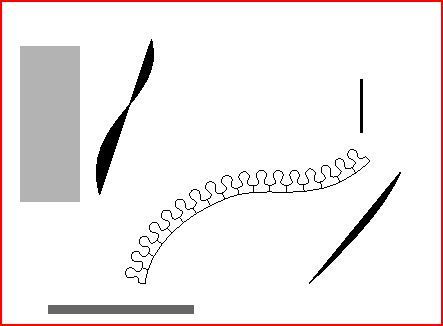
\includegraphics[width=\linewidth]{example}
%   \caption{Illustration of \texttt{\bslash cooltooltip} arguments}
%   \label{fig:ctip-arguments}
% \end{figure}
%
% Because \cool\ uses \LaTeX's |\label|\slash|\pageref| mechanisms for
% accurately determining the current page, documents built using \cool\
% will need to be run through |pdflatex| at least twice.  (|pdflatex|
% will issue the standard ``\texttt{Rerun to get cross-references
% right}'' message as a reminder.)
%
% \begin{decl}
%   \texttt{\string\cooltooltiptoggle} \marg{text}
% \end{decl}
% \bgroup
%   \def\PrintDescribeMacro#1{}
%   \DescribeMacro{\cooltooltiptoggle}
% \egroup
%
% The popup mechanism used by \cool\ is extremely fragile.  \cool\ has
% to manually transfer focus among the hyperlink, popup, and a per-page
% invisible form field.  (See Section~\ref{sec:widgets} for details and
% an explanation of why this trickery is necessary.)  If the browser
% window is so small that the popup overlaps the mouse pointer, the
% popup will flicker rapidly and impede the use of the hyperlink.
% Because this behavior is disturbing to readers of the document, the
% author may want to provide the reader with the ability to disable
% popups.
%
% The |\cooltooltiptoggle| command converts its \meta{text} argument to
% a toggle button.  Pressing the button suppresses all popups in the
% document.  Pressing it again re-enables popups.
%
%
% \StopEventually{^^A
% \section{Future work}
%
% There's unlikely to be any future work on \cool; consider it to be a
% ``dead'' package.  Yes, I know that someone will want a
% \texttt{dvipdfm} port and someone else will want finer-grained control
% over which of \meta{subject}, \meta{message}, \meta{\acro{url}}, and
% \meta{tooltip} are utilized and a third person will request a less
% sloppy implementation of the code.  However, I wrote \cool\ primarily
% as a one-time-use package for my personal use; I needed a way to
% implement fancy popups for my Visual \LaTeX\ FAQ document and
% initially had no intention of distributing the popup mechanism as a
% separate package.  If you find \cool\ useful in its current form,
% that's great.  If not, then you're on your own for fixing it; I don't
% plan on spending any significant time maintaining the package.
%
%
% \section{License agreement}
% \label{sec:license}
%
% \begin{center}
% Copyright \textcopyright{} 2006
% by Scott Pakin \texttt{<scott+ctip@pakin.org>}
% \end{center}
%
% \noindent
% This file may be distributed and/or modified under the conditions of
% the \LaTeX{} Project Public License, either version~1.3b of this
% license or (at your option) any later version.  The latest version of
% this license is in \url{http://www.latex-project.org/lppl.txt} and
% version~1.3b or later is part of all distributions of \LaTeX{} version
% 2006/01/07 or later.
% }
%
% \section{Implementation}
% \label{sec:implementation}
%
% This section presents the commented \LaTeXe\ source code for the
% \cool\ package.  Each cool tooltip is implemented in terms of two
% \acro{pdf} \pdfterm{Annot} objects.  The popup is a \pdfterm{Text}
% annotation with an invisible appearance.  The popup trigger/tooltip is
% both a \pdfterm{Widget} annotation and \pdfterm{Btn} pushbutton field.
% JavaScript code implements the popup open/close logic.  For
% compatibility with \acro{pdf} browsers that don't support
% \pdfterm{Widget} annotations we also include an ordinary
% \pdfterm{Link} annotation.
%
% Section~\ref{sec:implementation} is structured as follows.
% Section~\ref{sec:acroform} marks the document as a \acro{pdf} form,
% which is necessary for using fields and widgets.
% Section~\ref{sec:text} defines macros for creating a \pdfterm{Text}
% annotation, \cool's popup mechanism.  Most of \cool's behavior is
% defined in Section~\ref{sec:widgets}.  All \acro{pdf}
% fields/\pdfterm{Widget}s are specified in that section.  The
% |\cooltooltip| command proper is defined in
% Section~\ref{sec:user-commands}.  Finally,
% Section~\ref{sec:sanity-checks} includes a tiny amount of extra code
% to verify that the document is being built under pdf\LaTeX\@.  If not,
% it disables all \cool\ functionality but enables the document to build
% without it.
%
% \bigskip
%
% Because \cool\ works only with pdf\LaTeX\ and only in \acro{pdf} mode,
% we load the \textsf{ifpdf} package up front to simplify testing for
% that case.
%    \begin{macrocode}
\RequirePackage{ifpdf}
%    \end{macrocode}
%
%
% \subsection{\pdfterm{AcroForm} construction}
% \label{sec:acroform}
%
% \acro{pdf} requires that all top-level form fields be pointed to by an
% \pdfterm{AcroForm} entry in the catalogue.  We therefore have to keep
% track of all of our form fields.
%
% \begin{macro}{ctip@form@fields}
% Define a list of ``\meta{object}~|0 R|'' elements.
%    \begin{macrocode}
\newcommand*{\ctip@form@fields}{}
%    \end{macrocode}
% \end{macro}
%
% At the end of the document we need to export the final value of
% |\ctip@form@fields| as an \pdfterm{AcroForm}.
%    \begin{macrocode}
\ifpdf
  \AtEndDocument{%
    \immediate\pdfobj {
      <<
        /Fields [\ctip@form@fields]
        /NeedAppearances true
      >>
    }%
%    \end{macrocode}
%    \begin{macrocode}
    \pdfcatalog {
      /AcroForm \the\pdflastobj\space 0 R
    }%
  }
\fi
%    \end{macrocode}
%
%
% \subsection{\pdfterm{Text} annotation construction}
% \label{sec:text}
%
% \begin{macro}{\ctip@empty@icon}
% Define an empty \pdfterm{XForm} object to use as an invisible icon for
% the \pdfterm{Text} annotation.
%    \begin{macrocode}
\ifpdf
  \setbox\@tempboxa=\hbox{}
  \immediate\pdfxform\@tempboxa
  \edef\ctip@empty@icon{\the\pdflastxform}
\fi
%    \end{macrocode}
% \end{macro}
%
% \begin{macro}{\ctip@tip@number}
% Keep track of the current tip number.  This is necessary for
% generating unique object names.
%    \begin{macrocode}
\newcommand*{\ctip@tip@number}{0}
%    \end{macrocode}
% \end{macro}
%
% \begin{macro}{\ctip@make@Text}
% Create a \pdfterm{Text} annotation with a given color~(|#1|, optional),
% subject~(|#2|), and content string~(|#3|) and an invisible icon.  This
% annotation is what will be popped up when the pointer enters the
% associated \pdfterm{Widget}.
%    \begin{macrocode}
\newcommand*{\ctip@make@Text}[3][0 1 0]{%
  \pdfannot width 0pt height 0pt depth 0pt {
    /Subtype /Text
    /C [#1]
    /Subj (#2)
    /Contents (#3)
    /NM (ctip Text \ctip@tip@number)
    /AP <<
      /N \ctip@empty@icon\space 0 R
      /D \ctip@empty@icon\space 0 R
      /R \ctip@empty@icon\space 0 R
    >>
    /Open false
  }%
}
%    \end{macrocode}
% \end{macro}
%
%
% \subsection{\pdfterm{Widget} annotation construction}
% \label{sec:widgets}
%
% The \pdfterm{Widget}s in this section are also \acro{pdf} pushbutton
% fields.  \acro{pdf} supports merging the two object dictionaries
% because their keys are disjoint.
%
% \begin{macro}{\ctip@current@page}
% Store the page number on which a \pdfterm{Widget} is finally placed.
%    \begin{macrocode}
\newcommand*{\ctip@current@page}{1}
%    \end{macrocode}
% \end{macro}
%
% \begin{macro}{\ctip@last@invis}
% Keep track of the page number on which we last placed an invisible
% \pdfterm{Widget}.
%    \begin{macrocode}
\newcommand*{\ctip@last@invis}{0}
%    \end{macrocode}
% \end{macro}
%
% \begin{macro}{\ctip@label}
% The \pkgname{amsmath} package redefines |\label| within its equation
% environments.  We need access to the original |\label| so we store a
% copy in |\ctip@label|.
%    \begin{macrocode}
\let\ctip@label=\label
%    \end{macrocode}
% \end{macro}
%
% \begin{macro}{\ctip@update@pagenum}
% We can't reliably use |\thepage| to get the current page number
% (cf.~\url{http://www.tex.ac.uk/cgi-bin/texfaq2html?label=wrongpn}).
% Hence, we exploit the |\label|\slash|\pageref| mechanism to get an
% accurate page number.  |\ctip@update@pagenum| creates a label (based
% on Section~\ref{sec:text}'s |\ctip@tip@number|) then sets
% |\ctip@current@page| to the page on which the label occurs.
%    \begin{macrocode}
\newcommand*{\ctip@update@pagenum}{%
%    \end{macrocode}
% \begin{macro}{\ctip@refname}
% Using |\label| to define a label \meta{label name} implicitly defines
% a macro called |\r@|\meta{label name}.  That macro is |\relax| the
% first time |pdflatex| is run and thereafter expands to some number of
% values, the second of which is the label's page number.
%    \begin{macrocode}
  \ctip@label{ctip:tip:\ctip@tip@number}%
  \expandafter\let\expandafter\ctip@refname
    \csname r@ctip:tip:\ctip@tip@number\endcsname
  \@ifundefined{ctip@refname}{%
%    \end{macrocode}
% The first time through we use |\thepage| as an estimate for the
% correct page number.
%    \begin{macrocode}
    \xdef\ctip@current@page{\thepage}%
  }{%
%    \end{macrocode}
% On subsequent runs we extract the second (page number) argument and
% discard the rest.
%    \begin{macrocode}
    \def\ctip@secondofN##1##2##3!{%
      \xdef\ctip@current@page{##2}%
    }%
    \expandafter\ctip@secondofN\ctip@refname!%
  }%
}
%    \end{macrocode}
% \end{macro}
% \end{macro}
%
% \begin{macro}{\ctip@make@invisible@Widget}
% For a \pdfterm{Widget} to return focus to the ``background'' it really
% returns focus to an \emph{invisible} \pdfterm{Widget}.  We need only
% one invisible \pdfterm{Widget} per page for this trick to work.
%    \begin{macrocode}
\newcommand*{\ctip@make@invisible@Widget}{%
  \pdfannot width 0pt height 0pt depth 0pt {
    /Subtype /Widget
    /FT /Btn
    /T (ctip invisible Widget \ctip@current@page)
    /DA (/Helv 10 Tf 0 0 0 rg)
    /Ff 65536
    /F 2
%    \end{macrocode}
% Sometimes, for various focusing trickery to work, the invisible
% \pdfterm{Widget} has to be made visible temporarily.  We therefore
% define an action that makes the \pdfterm{Widget} invisible again as
% soon as it receives the input focus.
%    \begin{macrocode}
    /AA <<
      /Fo <<
        /Type /Action
        /S /JavaScript
        /JS (event.target.display = display.hidden)
     >>
    >>
  }%
}
%    \end{macrocode}
% \end{macro}
%
% \begin{macro}{\ctip@content@box}
% The \pdfterm{Widget}'s visual content is stored as a \TeX\ box.
%    \begin{macrocode}
\newsavebox{\ctip@content@box}
%    \end{macrocode}
% \end{macro}
%

% \begin{macro}{\ctip@unfocus@js}
% Although a \acro{pdf} field can grab the input focus using the
% JavaScript |setFocus()| method, there's no mechanism in \acro{pdf}~1.6
% to explicitly reset the input focus to the page.  The reason we want
% to clear the input focus is that the Page~Up and Page~Down keys
% function as expected only when none of the fields have the focus.
% |\ctip@unfocus@js| expands to some JavaScript code that implicitly
% resets the input focus.  The trick is to make an invisible
% \pdfterm{Widget} temporarily visible, give it the focus, and let its
% focus~(|Fo|) action make the \pdfterm{Widget} invisible again.
% Because an invisible \pdfterm{Widget} apparently can't retain the
% input focus, the focus is reset to the page.
%    \begin{macrocode}
\newcommand*{\ctip@unfocus@js}{%
  var ctipField =
    this.getField("ctip invisible Widget \ctip@current@page");
  ctipField.display = display.visible;
  ctipField.setFocus();
}
%    \end{macrocode}
% \end{macro}
%
% \begin{macro}{\ctip@enter@js}
% The |\ctip@enter@js| macro expands to some JavaScript code to execute
% when the mouse pointer enters the (visible) \pdfterm{Widget}.  The
% code instructs the associated \pdfterm{Text} annotation to open.  If
% the global JavaScript variable |ctip_disable_popups| is set to |true|
% then |\ctip@enter@js| does nothing.
%    \begin{macrocode}
\newcommand*{\ctip@enter@js}{%
  if (!global.ctip_disable_popups) {
    var ctipText =
      this.getAnnot(this.pageNum, "ctip Text \ctip@tip@number");
    ctipText.popupOpen = true;
    \ctip@unfocus@js
  }
}
%    \end{macrocode}
% \end{macro}
%
% \begin{macro}{\ctip@exit@js}
% The |\ctip@exit@js| macro expands to some JavaScript code to execute
% when the mouse pointer exits the (visible) \pdfterm{Widget}.  The code
% instructs the associated \pdfterm{Text} annotation to close.  The
% problem is that it doesn't close immediately but rather waits until
% focus leaves the \pdfterm{Text} annotation.  (Opening the annotation
% apparently gives it focus.)  Hence, we explicitly change the focus to
% the associated invisible \pdfterm{Widget} annotation to force the
% \pdfterm{Text} annotation to close immediately.  Because the invisible
% \pdfterm{Widget} is invisible it can't steal the input focus from the
% page and thereby prevent the Page~Up and Page~Down keys from
% functioning properly.  If the global JavaScript variable
% |ctip_disable_popups| is set to |true| then |\ctip@exit@js| does
% nothing.
%    \begin{macrocode}
\newcommand*{\ctip@exit@js}{%
  if (!global.ctip_disable_popups) {
    var ctipText =
      this.getAnnot(this.pageNum, "ctip Text \ctip@tip@number");
    ctipText.popupOpen = false;
    \ctip@unfocus@js
  }
}
%    \end{macrocode}
% \end{macro}
%
% \begin{macro}{\ctip@make@Widget}
% Create a \pdfterm{Widget} annotation which represents a pushbutton
% field.  |\ctip@make@Widget| expects |\ctip@content@box| to have the
% desired height, width, and depth of the \pdfterm{Widget}.  The
% arguments to |\ctip@make@Widget| are the link color~(|#1|, optional),
% the \acro{url} to link to~(|#2|), the tooltip to display~(|#3|).
%    \begin{macrocode}
\newcommand*{\ctip@make@Widget}[3][0 1 0]{%
%    \end{macrocode}
% Prepare to make the \pdfterm{Widget} annotation the same size as
% |\ctip@content@box| plus an |\fboxsep|$+$|\fboxrule|'s worth of space
% on each of its four sides.
%    \begin{macrocode}
  \setlength{\@tempdima}{\wd\ctip@content@box}%
  \addtolength{\@tempdima}{\fboxsep}%
  \setlength{\@tempdimb}{\ht\ctip@content@box}%
  \addtolength{\@tempdimb}{0.5\fboxsep}%
  \setlength{\@tempdimc}{\dp\ctip@content@box}%
  \addtolength{\@tempdimc}{0.5\fboxsep}%
  \hspace*{-0.5\fboxsep}%
%    \end{macrocode}
% \begin{macro}{\ctip@action@object}
% Create a separate \pdfterm{Action} object because we intend to use it
% in both the \pdfterm{Widget} annotation and in a \pdfterm{Link}
% annotation.  (See below.)
%    \begin{macrocode}
  \immediate
  \pdfobj {
    <<
      /Type /Action
      /S /URI
      /URI (#2)
    >>
  }%
  \edef\ctip@action@object{\the\pdflastobj\space 0 R}%
%    \end{macrocode}
% \end{macro}
% For compatibility with xpdf, which---as of this writing---does not
% support \pdfterm{Widget} annotations, we put a \pdfterm{Link}
% annotation behind the \pdfterm{Widget} annotation.
%    \begin{macrocode}
  \makebox[0pt][l]{%
%    \end{macrocode}
% Because |\fboxrule| is rounded down when used as a \pdfterm{Border}
% width we (locally) increment it by $\sim 1$ to get it to round up
% instead.
%    \begin{macrocode}
    \advance\fboxrule by 0.9999pt
    \pdfannot width \@tempdima
              height \@tempdimb
              depth \@tempdimc {
      /Subtype /Link
      /A \ctip@action@object
      /Border [0 0 \strip@pt\fboxrule]
      /C [#1]
    }%
  }%
%    \end{macrocode}
% We now create a \pdfterm{Widget} annotation, which is placed directly
% atop the \pdfterm{Link} annotation.
%    \begin{macrocode}
  \pdfannot width \@tempdima
            height \@tempdimb
            depth \@tempdimc {
    /Subtype /Widget
    /FT /Btn
    /T (ctip Field \ctip@tip@number)
%    \end{macrocode}
% Acrobat~7.0, at least, displays the ``alternate field
% name''~(\pdfterm{TU}) as a tooltip.
%    \begin{macrocode}
    /TU (#3)
%    \end{macrocode}
% We're obligated to include a default appearance string~(\pdfterm{DA})
% even though we don't really need it here.
%    \begin{macrocode}
    /DA (/Helv 10 Tf 0 0 0 rg)
%    \end{macrocode}
% Set bit~17 ($2^{17-1}$) of the field flags~(\pdfterm{Ff}) to indicate
% that this is a pushbutton---as opposed to a radio button or check box.
%    \begin{macrocode}
    /Ff 65536
%    \end{macrocode}
% Honor |\fboxrule| as the width of the link border.
%    \begin{macrocode}
    /BS <<
      /Type /Border
      /W \strip@pt\fboxrule
    >>
%    \end{macrocode}
% Define an appearance.
%    \begin{macrocode}
    /MK <<
      /BC [#1]
      /TP 1
    >>
%    \end{macrocode}
% Create an additional actions~(\pdfterm{AA}) dictionary.  This is where
% all of the popup magic is defined.
%    \begin{macrocode}
    /AA <<
%    \end{macrocode}
% When the mouse pointer enters the \pdfterm{Widget} we tell our
% associated \pdfterm{Text} annotation to open.
%    \begin{macrocode}
      /E <<
        /Type /Action
        /S /JavaScript
        /JS (\ctip@enter@js)
      >>
%    \end{macrocode}
% When the mouse pointer exits the \pdfterm{Widget} we tell our
% associated \pdfterm{Text} annotation to close.
%    \begin{macrocode}
      /X <<
        /Type /Action
        /S /JavaScript
        /JS (\ctip@exit@js)
      >>
%    \end{macrocode}
% When the user clicks on the \pdfterm{Widget} we relinquish the input
% focus and launch the specified \acro{url}.
%    \begin{macrocode}
      /U <<
        /Type /Action
        /S /JavaScript
        /JS (\ctip@unfocus@js)
        /Next \ctip@action@object
      >>
    >>
  }
%    \end{macrocode}
% Now that the \pdfterm{Widget} is defined we need to append an object
% reference for it to |\ctip@form@fields| so we can add that to the
% document's \pdfterm{AcroForm}.
%    \begin{macrocode}
  \xdef\ctip@form@fields{\ctip@form@fields\space\the\pdflastannot\space 0 R}
}
%    \end{macrocode}
% \end{macro}
%
%
% \subsection{User commands}
% \label{sec:user-commands}
%
% \begin{macro}{\cooltooltip}
% The user can create a cool tooltip by invoking |\cooltooltip| with the
% popup color~(|#1|, optional), the link color~(|#2|, optional), the
% subject of the popup~(|#3|), the string to display in the
% popup~(|#4|), the \acro{url} to link to~(|#5|), the tooltip to
% display~(|#6|), and the text that will activate the
% tooltip/popup~(|#7|).
%    \begin{macrocode}
\DeclareRobustCommand{\cooltooltip}[1][0 1 0]{%
  \def\ctip@popup@color{#1}%
  \ctip@cooltooltip@i
}
%    \end{macrocode}
% \end{macro}
%
% \begin{macro}{\ctip@cooltooltip@i}
% This is where everything gets called.  Upon entry, |\ctip@popup@color|
% is already defined as the popup color (and default color for the
% link).
%    \begin{macrocode}
\newcommand*{\ctip@cooltooltip@i}[6][\ctip@popup@color]{%
%    \end{macrocode}
% Store into |\ctip@content@box| the visual appearance of the link.
%    \begin{macrocode}
  \savebox{\ctip@content@box}{#6}%
%    \end{macrocode}
% Increase the cool tooltip number.  |\ctip@tip@number| is used by
% |\ctip@make@Widget|, |\ctip@make@Text|, and |\ctip@update@pagenum|.
%    \begin{macrocode}
  \@tempcnta=\ctip@tip@number
  \advance\@tempcnta by 1
  \xdef\ctip@tip@number{\the\@tempcnta}%
%    \end{macrocode}
% Determine if we're on a new page and therefore need to create another
% invisible \pdfterm{Widget}.
%    \begin{macrocode}
  \ctip@update@pagenum
  \@tempcnta=\ctip@last@invis
  \@tempcntb=\ctip@current@page
  \ifnum\@tempcnta<\@tempcntb
    \ctip@make@invisible@Widget
    \xdef\c@ctip@last@invis{\ctip@current@page}%
  \fi
%    \end{macrocode}
% Place a \pdfterm{Widget} and its associated \pdfterm{Text} popup but
% without occupying any space on the page (as far as \TeX\ can
% determine).
%    \begin{macrocode}
  \makebox[0pt][l]{%
    \ctip@make@Widget[#1]{#4}{#5}%
    \makebox[\paperwidth][r]{%
      \ctip@make@Text[\ctip@popup@color]{#2}{#3}%
    }%
  }%
%    \end{macrocode}
% Render the link contents that we stored earlier.
%    \begin{macrocode}
  \usebox{\ctip@content@box}%
}
%    \end{macrocode}
% \end{macro}
%
% \begin{macro}{\cooltooltiptoggle}
% Cool tooltips are rather kludgy in the way that they manipulate
% \acro{pdf} annotation state and transfer focus from annotation to
% annotation.  Because this kludginess can lead to strange interactive
% behavior we provide the author with a |\cooltooltiptoggle| macro which
% creates a button to disable/enable the \cool\ popup mechanism.  The
% sole argument to |\cooltooltiptoggle| is the button text.
%    \begin{macrocode}
\DeclareRobustCommand{\cooltooltiptoggle}[1]{%
  \savebox{\ctip@content@box}{#1}%
  \makebox[0pt][l]{%
    \pdfannot width \wd\ctip@content@box
              height \ht\ctip@content@box
              depth \dp\ctip@content@box {
      /Subtype /Link
      /Border [0 0 0]
      /A <<
        /Type /Action
        /S /JavaScript
        /JS (
          global.ctip_disable_popups = !global.ctip_disable_popups;
          var ctipField;
          var i;
          for (i=1; (ctipField=this.getField("ctip Field " + i)); i++)
            ctipField.display =
              global.ctip_disable_popups ? display.hidden : display.visible;
        )
      >>
    }%
  }%
  \usebox{\ctip@content@box}%
}
%    \end{macrocode}
% \end{macro}
%
%
% \subsection{Sanity checks}
% \label{sec:sanity-checks}
%
% Complain---but attempt to continue---if we're not running pdf\LaTeX\
% in \acro{pdf} mode.
%    \begin{macrocode}
\RequirePackage{ifpdf}
\ifpdf
\else
  \PackageWarning{cooltooltips}{%
    Not running pdfLaTeX in PDF mode; disabling cooltooltips%
  }
  \renewcommand*{\ctip@cooltooltip@i}[6][]{\mbox{#6}}
\fi
%    \end{macrocode}
%
%
% \Finale
\endinput
